%
% CHAPTER - Philosophy of Science
%

\chapterimage{LHC.pdf} % Chapter heading image

\chapter{Analysis of Science}
\label{chap:philosophy-science}

\begin{quote}
\begin{flushright}
\emph{Science may be regarded as the art of data compression.}\\
Li \& Vitányi
\end{flushright}
\end{quote}
\bigskip

{\color{red} TODO: Write this introduction}

In this chapter we will use our theory of nescience to study our current scientific knowledge

We will see how he can approximate the concept of nescience in practice. The concept of surfeit will be based, as it was described in Chaper XX, on the concept of redundancy, and redundancy will be computed in practice based on starndar text compressors.

A historical analyis of the evolution of nescience is also covered in the chapter.

At the end of the chapter we will extend the analysis from individual research topic to research areas, in order to understand 

%
% Section: Describing Current Knowledge
%
\section{Existing Knowledge}

According to the theory of nescience, the evaluation of human knowledge begins by selecting a specific set of entities we want to understand. Within our theory, we cannot use universal sets that include every possible entity, whether known or unknown. This is because universal sets lead to logical paradoxes, such as Cantor's theorem, which shows that the set of all possible subsets of a set has a strictly greater cardinality than the set itself, and Russell's paradox, which concerns sets that are not members of themselves (see Section XX). Therefore, in this chapter, since our aim is to assess the current state of human knowledge, we will focus on the set of all entities that are already known and have been studied by science. These are the entities about which humanity has at least some information, making them suitable for analysis, as the set is finite.

The next step is to identify the best available encoding of the selected entities as representations, composed by data or facts, followed by determining the most accurate descriptions we have about them, such as models, theories, and laws. In the theory of nescience, we make a clear distinction between representations and descriptions because this separation helps us discover new knowledge—either by improving the representation or by finding a better description. However, when assessing the current state of our knowledge, we simplify the process by using only descriptions, allowing them to serve both as the description and the representation of an entity (see Section XX, which explains why descriptions can also serve as representations). This approach is appropriate because our goal is not to increase our knowledge but to evaluate its current status.

The descriptions used for the analysis of knowledge will be based on the collection of scientific pages from Wikipedia\index{Wikipedia}. Wikipedia is a free, collaborative online encyclopedia that allows anyone with internet access to create, edit, and update articles on a wide range of topics.  Launched in 2001, it aims to provide reliable, neutral, and verifiable information to the public, maintained by a global community of volunteer contributors. Several features make Wikipedia particularly suitable for our analysis of scientific knowledge: it maintains a transparent version history that tracks the evolution of content over time, supports collaborative validation through contributions from a global community which helps reduce individual bias, enforces citation requirements to ensure information is verifiable and sourced from authoritative references, offers broad and consistent coverage across scientific domains, and benefits from dynamic updating to incorporate new findings and corrections.

Wikipedia pages are written in the MediaWiki Markup Language, a simplified system for formatting text that allows users without technical knowledge of XHTML or CSS to easily edit articles. Before we can analyze the content of a scientific page, it is essential to remove all markup tags and formatting elements to isolate only the meaningful textual information. To achieve this, we employed an advanced Wikipedia Extractor utility that processes the articles and extracts the relevant text. In addition to stripping out the markup, the extractor was configured to eliminate other non-relevant elements, such as images, references, and lists, which do not contribute directly to our analysis of knowledge. A detailed explanation of the entire extraction and preparation process can be found in Appendix XXX, allowing any interested reader to reproduce the steps and ensure the consistency of the analysis.

{\color{red} Explain which articles have been removed and why.}

%
% Section: Measuring Knowledge
%
\section{Measuring Knowledge}

As we said in the previous section, for the purpose of evaluating our current knowledge in practice, we usually to use as encoding of a entity our current best description (recall Section XX that said that descritions are also representations). In this sense, since representation and descriptions are the same, inaccuracy would be zero, remaining miscoding and sufeit as our metrics of interest.

In order to evaluate the classification metrics proposed we have used the set of topics corresponding to the discipline of \emph{theory of computation}.

{\color{red} TODO: Repeat this analysis for all scientific topics, and then particularize for a cuple of scientific areas relevant for this book (e.g. theoretical computer science, philosophy of science.}

Also, and since these studied quantities, relevance, applicability, nescience and maturity, do not have the same scale, it is highly convenient to apply the following additional transformation: ???

\[
\mu_{t}^{,}=\frac{\mu_{t}-\min(\mu)}{\max(\mu)-\min(\mu)}
\]

where $\mu_t$ refers to the considered metric (nescience, relevance, ...). 

% Surfeit
\subsection{Surfeit}

{\color{red} TODO: briefly recall the concept of surfeit, our inability to compute it in practice, and the approximation of redundancy.}

As it was the case in Capter {\color{red} XXX} the Kolmogorov complexity of a page was estimated using the compressed version of the text. As compressed tool we have used the Unix \texttt{gzip}
utility, that it is based on a combination of the Lempel-Ziv LZ77 algorithm {\color{red} ref} and Huffman coding {\color{red} ref}. Figure \ref{fig:Nescience-of-Topics} shows a plot of nescience for all the topics after normalization.

{\color{red} TODO: This fugure is useless. Better use an histogram or a boxplot, or violin plot.}

{\color{red} TODO: Say something ingelligent based on what it is depicted in the figure.}

\begin{figure}[h]
\centering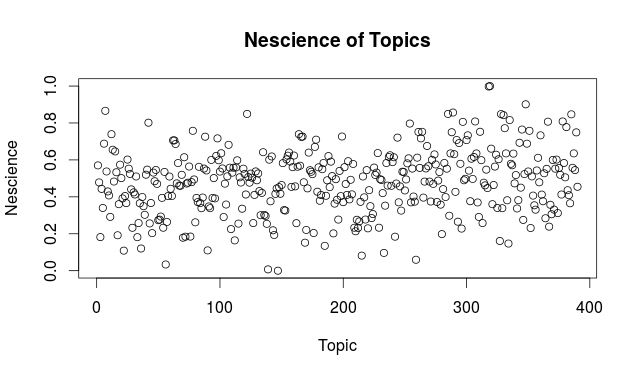
\includegraphics[scale=0.5]{NescienceTopics}
\caption{\label{fig:Nescience-of-Topics}Nescience of topics}
\end{figure}

{\color{red} Table \ref{tab:Nescience-of-topics} contain the ten topics with highest redundancy, and the normalized version of this number. The identification of the topics with highest nescience is even more controversial. Some authors would argue that the topics listed in the table are the least known topics in the area of theory of computation, like for example \emph{UML state machine} or \emph{Kleene's recursion theorem}. However the list includes very difficult to address topics, \emph{computability} and \emph{computability theory}, and hot research topics like the \emph{Kolmogorov structure function}. It is also remarkable that the list contains three related topics, \emph{analytical hierarchy}, \emph{arithmetical hierarchy} and \emph{hyperarithmetical theory}, suggesting that this is a highly unknown area of knowledge. An important point to mention is that our computed nescience is not directly proportional to the length of the article, and so, the list of the topics with the higher nescience does not mimic the list of the lengthiest articles.}

\begin{table}
\begin{centering}
\begin{tabular}{|c|c|c|}
\hline 
Topic & Nescience & Norm.\tabularnewline
\hline 
\hline 
Arithmetical hierarchy & 2.28 & 1.00\tabularnewline
\hline 
Analytical hierarchy & 2.28 & 1.00\tabularnewline
\hline 
Hyperarithmetical theory & 2.13 & 0.90\tabularnewline
\hline 
Kolmogorov struct. funct. & 2.08 & 0.87\tabularnewline
\hline 
Behavior of DEVS & 2.06 & 0.86\tabularnewline
\hline 
UML state machine & 2.05 & 0.85\tabularnewline
\hline 
Computability & 2.05 & 0.85\tabularnewline
\hline 
Kleene's recursion th. & 2.05 & 0.85\tabularnewline
\hline 
Computability theory & 2.04 & 0.84\tabularnewline
\hline 
Computation in the limit & 2.00 & 0.82\tabularnewline
\hline 
\end{tabular}
\par\end{centering}

\caption{\label{tab:Nescience-of-topics}Nescience of topics}
\end{table}

In practice, our definition of redundancy is problematic when we work with very short descriptions, since the compressed version of the text could be larger than the uncompressed version, given an negative nescience. This is still an open problem that must be addressed, perhaps by borrowing some techniques from the minimum description length principle.

The maturity of a topic is estimated based on the length of the Wikipedia article (only the text), and the length of the compressed version. Figure \ref{fig:Maturity-of-Topics} shows a plot of the maturity of the selected set of topics after the normalization process.

\begin{figure}[h]
\centering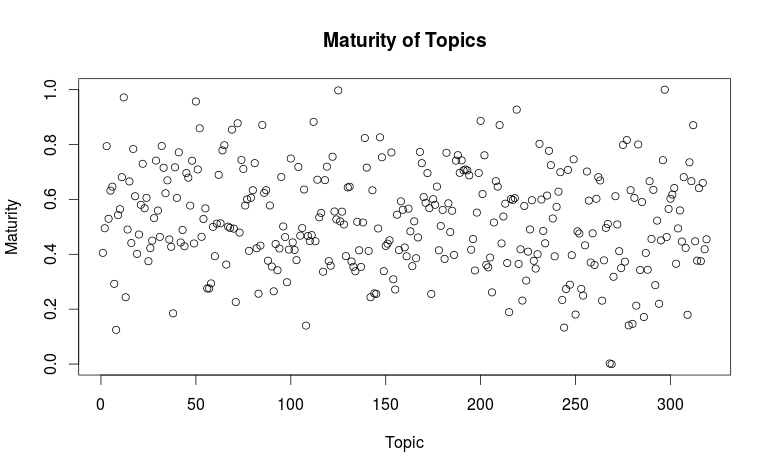
\includegraphics[scale=0.5]{MaturityTopics}
\caption{\label{fig:Maturity-of-Topics}Maturity of topics}
\end{figure}

Table \ref{tab:Maturity-of-Topics} contains the ten most relevant topics according to its maturity. For each topic it is shown the maturity and the normalized version of this number. Well classified topics, that is, topics that our intuition tell us that are well understood, could include \emph{Read-only right moving Turing machines}, \emph{Crossing sequence (Turing machines)}, and perhaps the \emph{P'' language}. Other topics that perhaps are misclassified include \emph{communication X-Machine}, \emph{Power DEVS}, \emph{MIPR}, and \emph{constraint automaton}.

\begin{table}
\begin{centering}
\begin{tabular}{|c|c|c|}
\hline 
Topic & Maturity & Norm.\tabularnewline
\hline 
\hline 
Carry operator & 5.34 & 1.00\tabularnewline
\hline 
Binade & 4.54 & 0.99\tabularnewline
\hline 
Comm. X-Machine & 3.01 & 0.97\tabularnewline
\hline 
PowerDEVS & 2.35 & 0.94\tabularnewline
\hline 
MPIR & 2.00 & 0.92\tabularnewline
\hline 
Constraint automaton & 1.84 & 0.90\tabularnewline
\hline 
RO right moving TM & 1.73 & 0.89\tabularnewline
\hline 
P'' & 1.71 & 0.89\tabularnewline
\hline 
Crossing sequence (TM) & 1.63 & 0.88\tabularnewline
\hline 
Microsoft Binary Format & 1.53 & 0.86\tabularnewline
\hline 
\end{tabular}
\par\end{centering}

\caption{\label{tab:Maturity-of-Topics}Maturity of topics}
\end{table}

% Subsection: Miscoding
\subsection{Miscoding}

%
% Section: Measuring Resarch Areas
%
\section{Measuring Research Areas}

Wikipedia's category system organizes articles into groups based on similar topics, facilitating navigation and information retrieval. Categories are interconnected, forming a flexible and overlapping structure rather than a strict hierarchy. Each category can contain multiple subcategories, and a subcategory may have multiple parent categories, allowing diverse classification schemes to coexist. However, care must be taken to avoid circular relationships, where a category indirectly becomes its own subcategory. This structure resembles a partially ordered set in mathematics and computer science. 

Articles are not typically placed in every logically relevant category; instead, they are categorized within the most specific applicable subcategory to maintain clarity. If membership in one category implies membership in another, the first should be designated as a subcategory of the second, ensuring a logical "is-a" relationship.

Category:Contents - This is the top level of Wikipedia's category system (it has no parent category).

Contents - Articles - Main topic classification - Academic disciplines - Science - Branches of science


In this section we analyze the interests of the different research areas, instead of the interest of individual topics. The areas analyzed are \emph{sociology} (Level 1 \emph{social sciences}, 6,004 topics),
\emph{biology} (Level 1 \emph{natural sciences}, 6,989 topics), \emph{computer science} (Level 1 \emph{applied sciences}, 1,331 topics), \emph{epistemology} (Level 1 \emph{cognitive science}, 4,268 topics), \emph{psychology} (Level 1 \emph{behavioral science}, 7,905 topics), \emph{chemistry} (Level 1 \emph{physical sciences}, 11,589 topics), and \emph{mathematics} (Level 1 \emph{formal sciences}, 4,688 topics).

Table \ref{tab:Interestingness-of-Areas-as-Tools} shows the average applicability and average maturity of each of the selected areas, and the average interestingness of each area as a source of interesting tools. The table largely fits our intuitive idea of which areas are more important as a source of tools: computer science is the area of highest interest, and sociology is the area with less interest. The only extrange elements is that epistemology appears as a source of very interesting tools, even more interesting, on average, than topics from mathematics (probably because it contains a large ratio of poorly written articles).

\begin{table*}
\begin{centering}
\begin{tabular}{|c|c|c|c|}
\hline 
Research Area & Applicability & Maturity & Tools\tabularnewline
\hline 
\hline 
Sociology & $1.00\times10^{-3}$ & $2.93\times10^{-3}$ & $3.09\times10^{-3}$\tabularnewline
\hline 
Biology & $9.20\times10^{-4}$ & $4.65\times10^{-3}$ & $4.74\times10^{-3}$\tabularnewline
\hline 
Chemistry & $3.11\times10^{-3}$ & $5.01\times10^{-3}$ & $5.90\times10^{-3}$\tabularnewline
\hline 
Psychology & $1.14\times10^{-3}$ & $6.91\times10^{-3}$ & $7.00\times10^{-3}$\tabularnewline
\hline 
Mathematics & $9.32\times10^{-3}$ & $9.47\times10^{-3}$ & $1.32\times10^{-2}$\tabularnewline
\hline 
Epistemology & $1.55\times10^{-3}$ & $1.75\times10^{-2}$ & $1.76\times10^{-2}$\tabularnewline
\hline 
Computer\_science & $9.93\times10^{-3}$ & $1.90\times10^{-2}$ & $2.15\times10^{-2}$\tabularnewline
\hline 
\end{tabular}
\par\end{centering}

\caption{\label{tab:Interestingness-of-Areas-as-Tools}Interestingness of Areas
as Tools}
\end{table*}

Finally, Table \ref{tab:Interestingness-of-Areas-as-Problems} shows the relevance and nescience of the selected areas, and their interest as a source of interesting problems. Again, the results largely match
our intuitive idea of which areas are less understood: sociology is the area with the highest number of interesting problems, and mathematics is the area with the lower number of problems.

\begin{table*}
\begin{centering}
\begin{tabular}{|c|c|c|c|}
\hline 
 & Relevance & Nescience & Problems\tabularnewline
\hline 
\hline 
Mathematics & $4.22\times10^{-2}$ & $3.51\times10^{-1}$ & $3.53\times10^{-1}$\tabularnewline
\hline 
Computer\_science & $2.35\times10^{-2}$ & $4.43\times10^{-1}$ & $4.44\times10^{-1}$\tabularnewline
\hline 
Chemistry & $5.95\times10^{-2}$ & $4.66\times10^{-1}$ & $4.70\times10^{-1}$\tabularnewline
\hline 
Biology & $3.85\times10^{-2}$ & $4.75\times10^{-1}$ & $4.77\times10^{-1}$\tabularnewline
\hline 
Psychology & $5.06\times10^{-2}$ & $5.28\times10^{-1}$ & $5.31\times10^{-1}$\tabularnewline
\hline 
Epistemology & $4.54\times10^{-2}$ & $5.30\times10^{-1}$ & $5.32\times10^{-1}$\tabularnewline
\hline 
Sociology & $4.21\times10^{-2}$ & $5.43\times10^{-1}$ & $5.44\times10^{-1}$\tabularnewline
\hline 
\end{tabular}
\par\end{centering}

\caption{\label{tab:Interestingness-of-Areas-as-Problems}Interestingness of Areas as Problems}
\end{table*}

%
% Section: The Evolution of Knowledge
%
\section{The Evolution of Knowledge}

{\color{red} TODO: Show the evolution of a research topic, preferably by using historical data from centuries ago, if not possible, using the evolution of a tipic given wikipedia.}

\begin{example}
In Figure \ref{fig:TheoreticalPerfectKnowledge} is depicted the evolution of a hypothetical research topic. Every point in the graph represents a new current best description for that topic (descriptions are ordered with respect to time). New descriptions could be based on novel theories that explain the topic, refinements over already existing ones, or on a reduction of the number of assumptions. In general, each new description should be shorter than the previous one. However, as we can see in the figure, it might happen that some descriptions are longer than its previous. That could be the case, for example, when we discover new facts that have to be taken into account by the theory. But the important thing is that nescience should decrease, in average, with time.
\end{example}

\begin{figure}[h]
\centering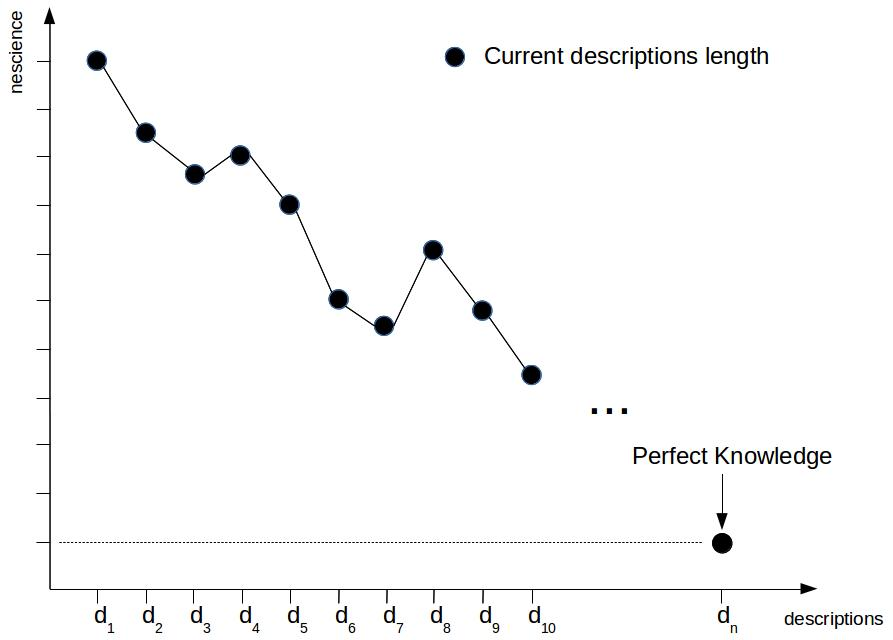
\includegraphics[scale=0.5]{TheoreticalPerfectKnowledge}
\caption{\label{fig:TheoreticalPerfectKnowledge}Evolution of Nescience}
\end{figure}

My hypothesis is that the nescience of topic descriptions decrease with time. On the contrary, the description of topics from pseudocience or religion does not decrease with time. This property, decrease with time is what distinguish science with respect other pseudosiences. I totally disagree with Feyerabend when he states that \emph{sicence has no special features that render it intrinsically superior to other kinds of knowledge such as ancient myths or voodoo}.

How does my view differ with respect to the point of view that states that "science is derived from facts"? Perhaps facts is what allow us to make shorter descriptions. But facts also can increase the length of a description.

Here I have to be very careful, becase if the description lenght of topics in phylosophy does not decrease with time, we should conclude that phylosophy is a pseudocience.

In order to understand a theory a background knowledge is assumed. What it is exactly that background is something that depends on the theory and the current undertanding of the theory.

\begin{example}
Suppose that the topic $t$ being studied is the concept of \emph{limit of a function}. The standard \emph{$\left(\epsilon,\delta\right)$-definition} of limit provided by Karl Weierstrass is:

\begin{eqnarray*}
\lim_{x\rightarrow c}f(x) & = & L\Leftrightarrow\forall\epsilon>0\:\exists\,\delta>0\,:\,\\
 &  & \forall x\,\left(0<\left|x-c\right|<\delta\Rightarrow\left|f(x)-L\right|<\epsilon\right)
\end{eqnarray*}


This definition has a length of 46 symbols, spaces not included\footnote{
For the sake of simplicity, we have computed the complexity of the
topic given the number of symbols, not the the length of its binary
representation, as it is required by our definition.}. The alternative \emph{infinitesimal definition} of limit, based
on non-standard calculus, is:

\[
\lim_{x\rightarrow c}f(x)=L\Leftrightarrow st(x)=c\Rightarrow st(f(x))=L
\]

where $st(\cdot)$ denotes the \emph{standard part function}, which \textquotedbl{}rounds off\textquotedbl{} each finite hyperreal%
\footnote{Nonstandard analysis deals primarily with the pair $\mathbb{R\subset^{\star}\mathbb{R}}$,
where hyperreals $^{\star}\mathbb{R}$ are an ordered field extension
of the reals $\mathbb{R}$, that contains infinitesimals in addition
to reals.%
} number to the nearest real. This second definition has a length of 31 symbols, and so, we say that our nescience of the concept of limit has decreased, since we were able to simplify the definition from a three quantifier block to a just one quantifier statement.

If the complexity $C_{t}$ of the concept of limit is less that 31 characters, then there must be possible to come up with a even shorter definition.\hfill{}$\square$
\end{example}

%
% Section: Knowledge by Category
%
\section{Knowledge by Category}

%
% Section: The Demarcation Problem
%
\section{The Demarcation Problem}

In this section, we propose a practical method, based on the theory of nescience, to address the demarcation problem\index{Demarcation problem}, specifically, the challenge of distinguishing scientific from non-scientific knowledge in real-world contexts. Although demarcation is a longstanding philosophical issue, our aim is not to conclusively solve this complex problem but rather to provide insights into its nature and outline potential paths toward future solutions through practical and operational methods.

For our experiments and analysis, we have selected six scientific topics and six pseudoscientific topics to evaluate our approach to the demarcation problem. Our analysis is based on the descriptions of these topics provided by Wikipedia and their associated \texttt{Talk} pages. As in previous analyses conducted in this chapter, we have preprocessed the Wikipedia pages by using the \texttt{wikitextparser} Python library to remove Wikimedia tags and other irrelevant elements such as tables and images.

The six scientific topics selected are: Climate Change (the long-term alteration of temperature and weather patterns), Graphene (a single-layer carbon material with extraordinary physical properties), Dark Matter (a hypothesized form of matter making up approximately 85\% of the universe), Deep Learning (a subset of machine learning using neural networks with multiple layers), Lithium-ion Battery (a type of rechargeable battery widely used for portable electronics and electric vehicles), and Brain–Computer Interface (a technology enabling direct communication between the brain and external devices). These scientific topics have been selected due to their intensive research activity over the past 20 years.

\begin{figure}[H]
\centering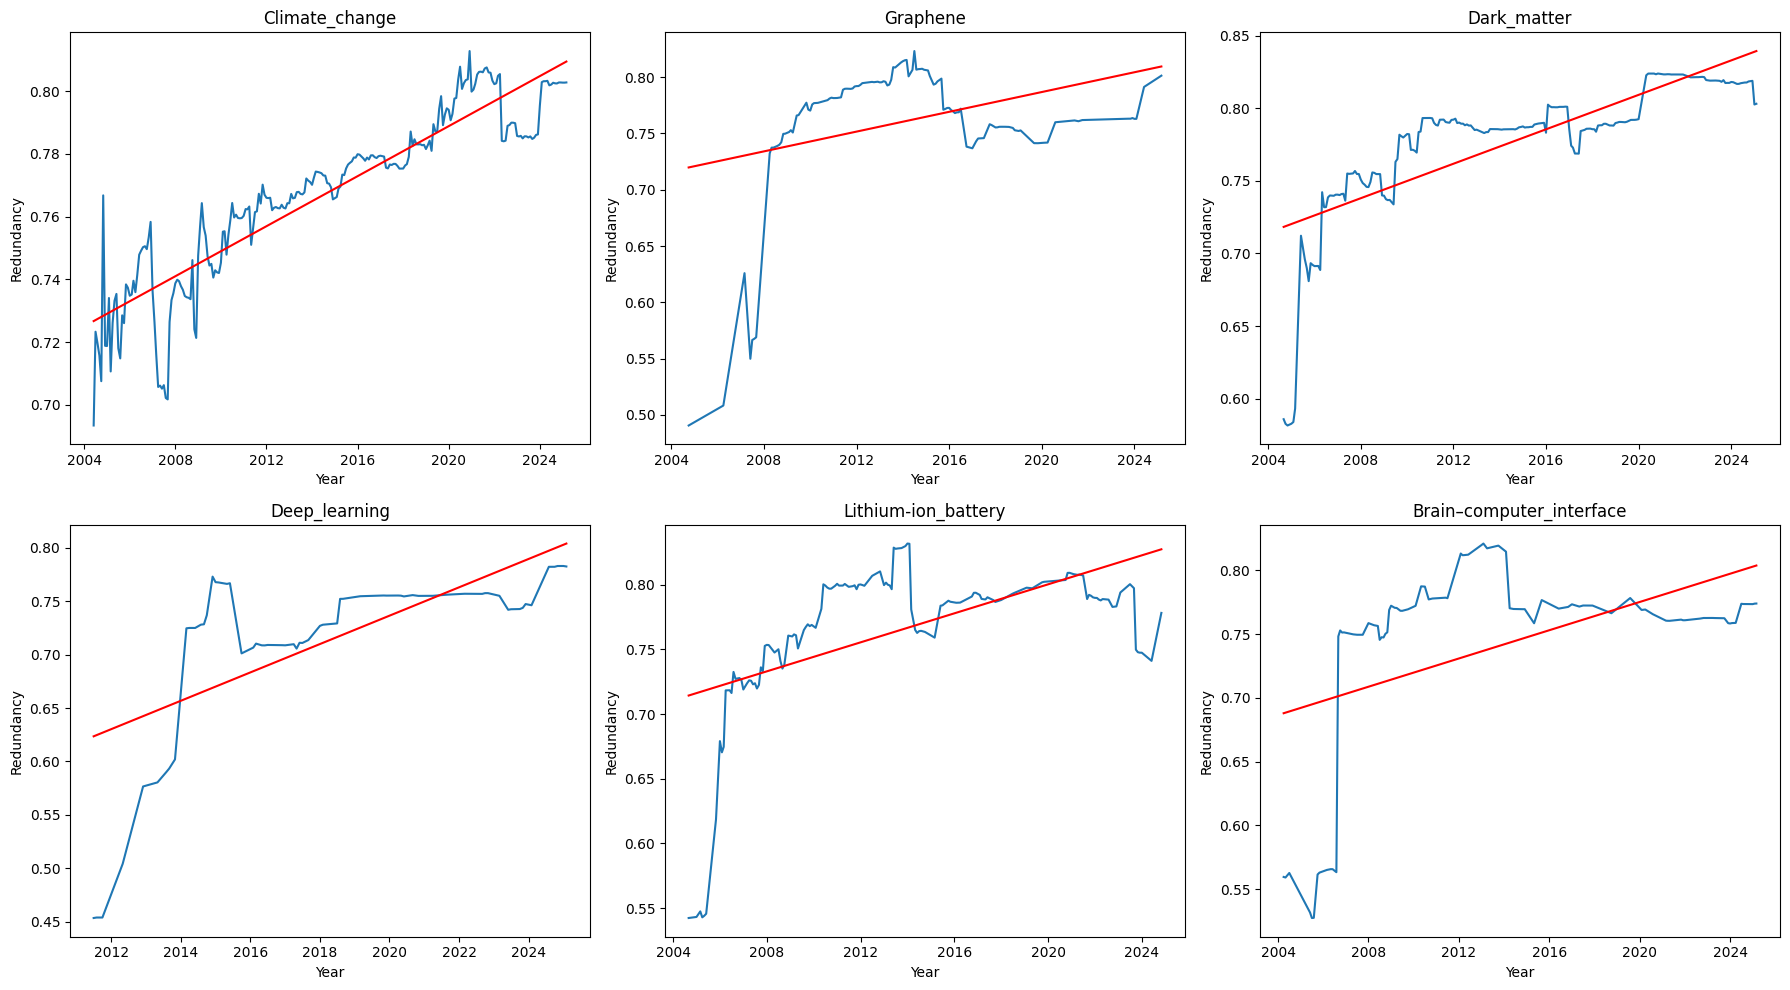
\includegraphics[scale=0.3]{RedundancySixScientific}
\caption{\label{fig:redundancy_six_scientific}Evolution of Redundancy in Scientific Topics}
\end{figure}

Redundancy, as an approximation of the concept of surfeit, is computed, as in the previous case, by comparing the ratio of the length of a text to its compressed version. Figure \ref{fig:redundancy_six_scientific} shows the evolution of redundancy for these selected scientific topics over the past 20 years. As observed, redundancy for these topics demonstrates an increasing trend, as confirmed by the computed regression line. Although one might generally expect redundancy to decrease as our understanding improves, new discoveries and emerging knowledge frequently necessitate additional details and explanations, thus increasing redundancy in descriptions.

\begin{figure}[H]
\centering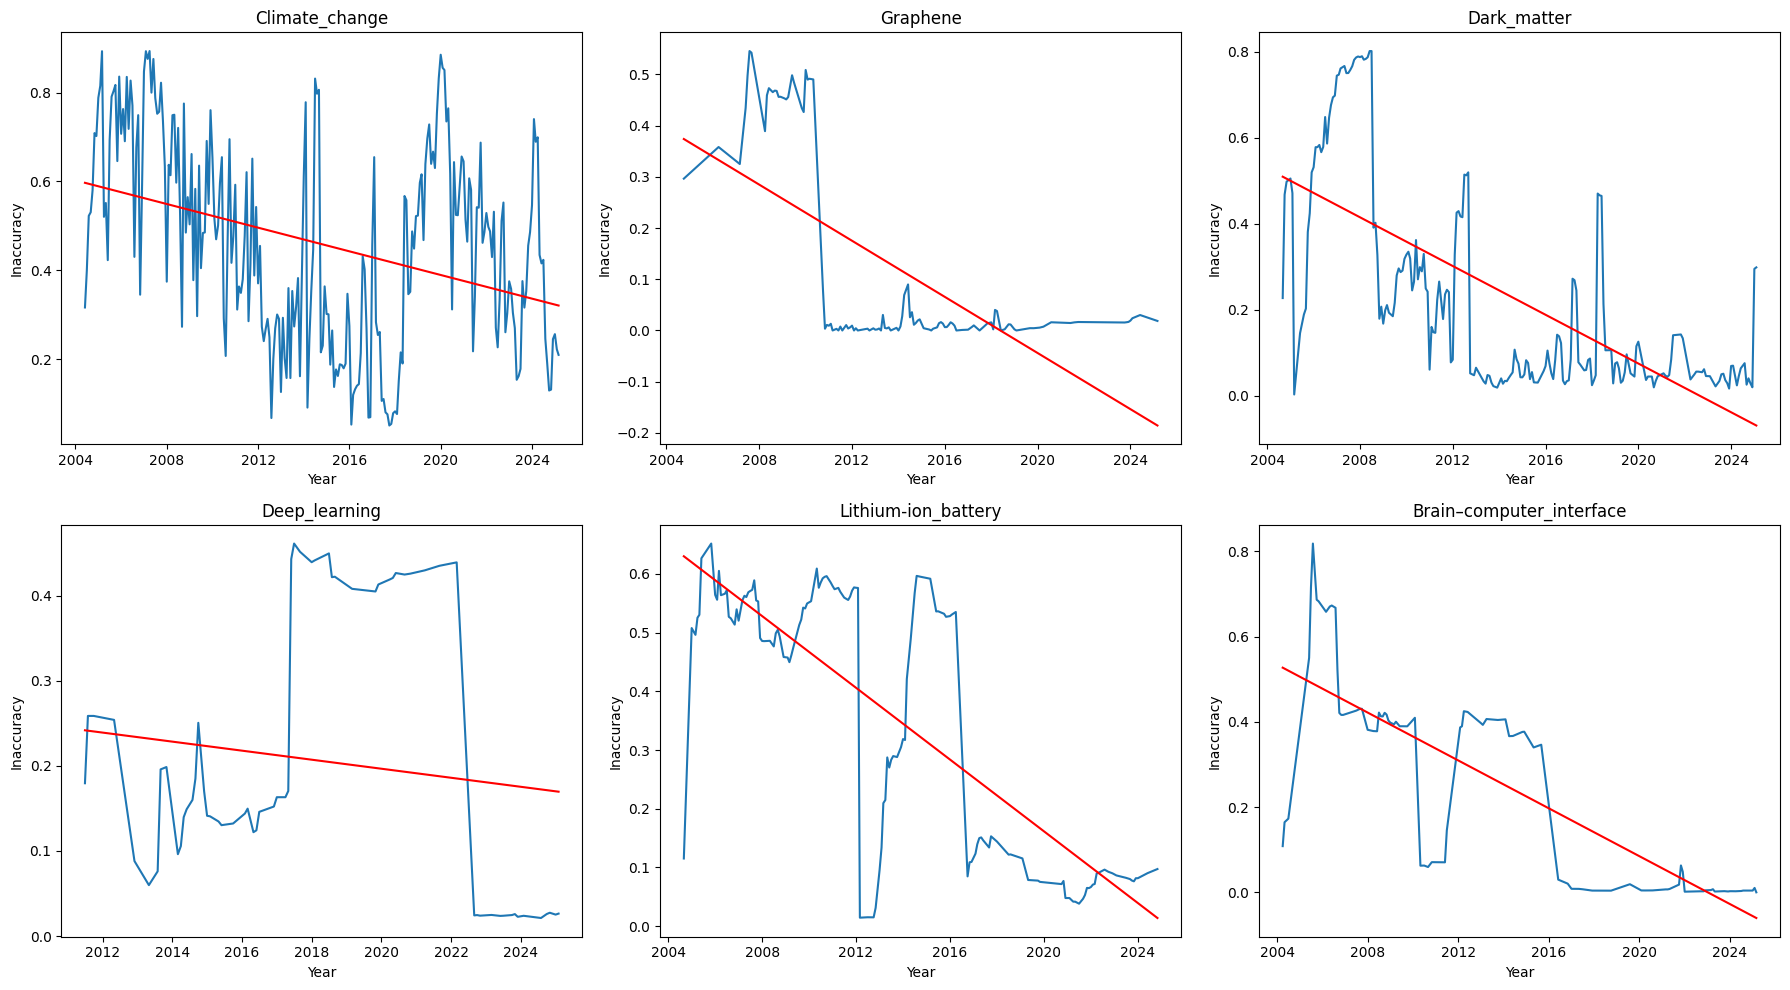
\includegraphics[scale=0.3]{InaccuracySixScientific}
\caption{\label{fig:inaccuracy_six_scientific}Evolution of Inaccuracy in Scientific Topics}
\end{figure}

Inaccuracy is computed based on the ratio length\_talk / (length\_talk + length\_article), where length\_talk represents the length of the Talk page for each topic, and length\_article is the length of the corresponding Wikipedia article, as done in the previous sections. Utilizing Talk pages is an effective method for approximating article inaccuracy since these pages typically contain discussions, disputes, and clarifications regarding inaccuracies or controversies in the articles. Figure \ref{fig:inaccuracy_six_scientific} illustrates the evolution of inaccuracies for the selected scientific topics, showing a clear decreasing trend across all topics.

\begin{figure}[H]
\centering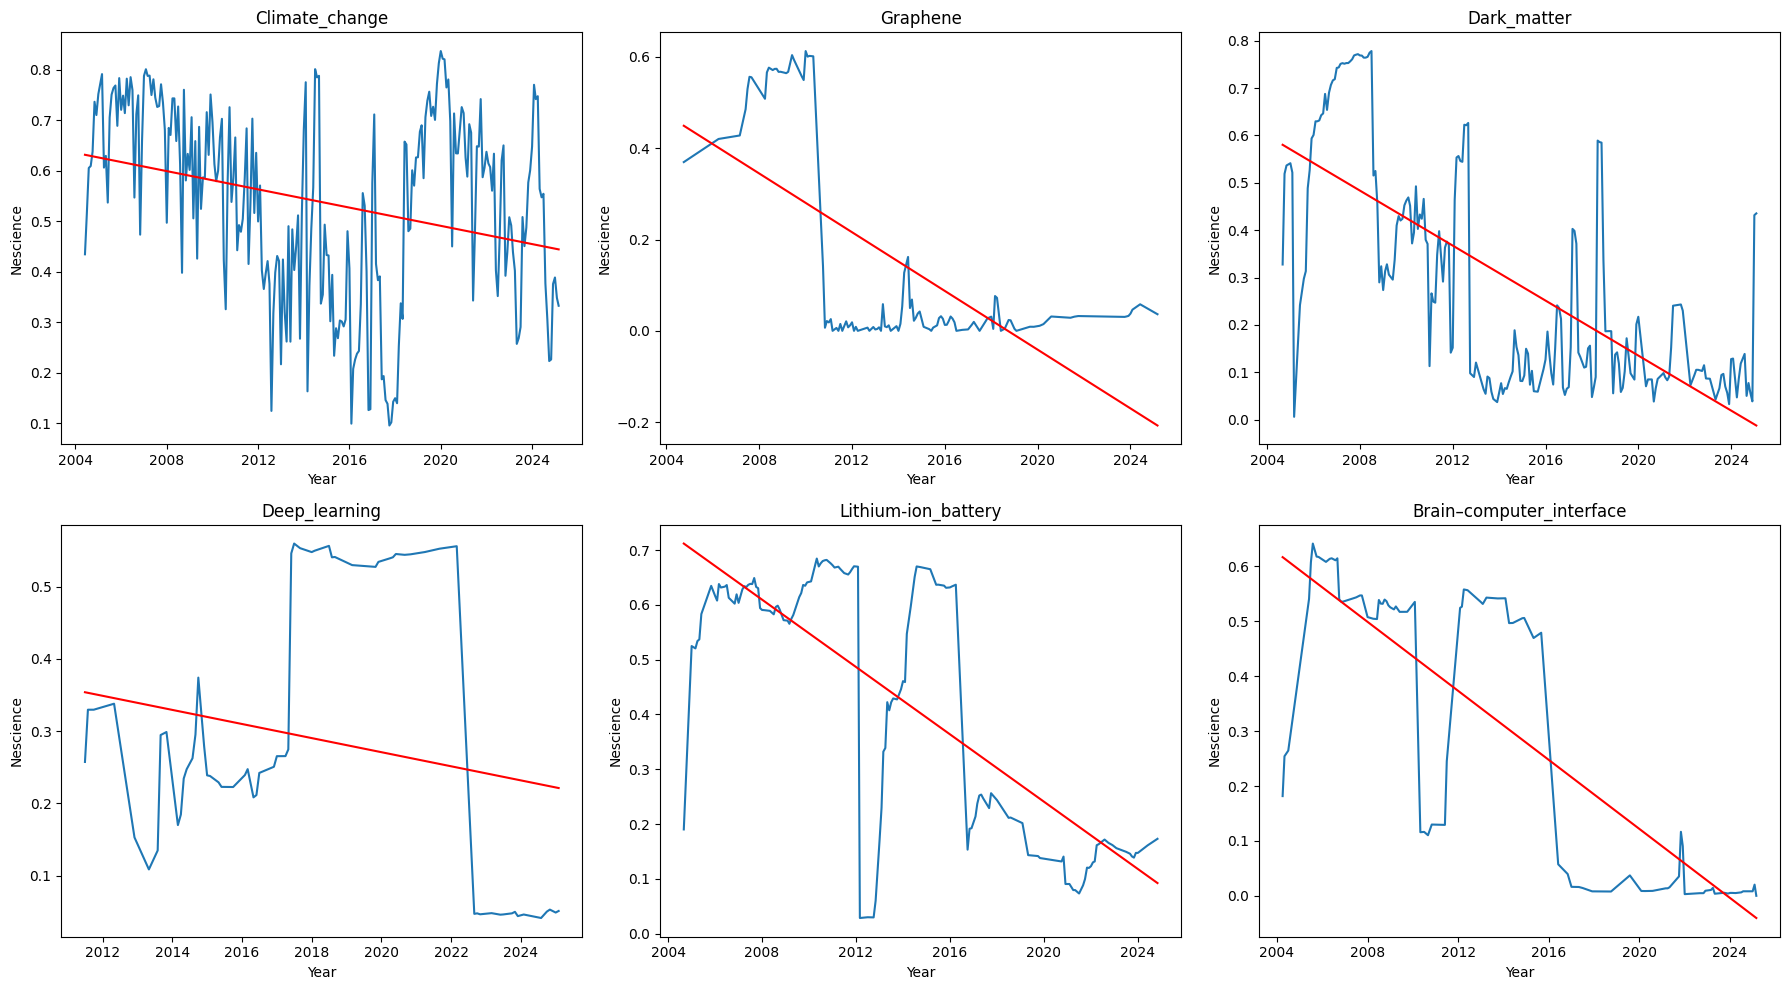
\includegraphics[scale=0.3]{NescienceSixScientific}
\caption{\label{fig:nescience_six_scientific}Evolution of Nescience in Scientific Topics}
\end{figure}

Finally, Figure \ref{fig:nescience_six_scientific} shows the evolution of nescience for all selected scientific topics, where nescience is estimated as the harmonic mean of the metrics of redundancy and inaccuracy. As depicted, despite the positive trend in redundancy, nescience exhibits a decreasing trend, suggesting our overall understanding of these topics improves over time.

Additionally, we have selected six pseudoscientific topics to further evaluate our demarcation method: Lunar Effect (the belief that lunar cycles influence human behavior), Water Memory (the claim that water retains a memory of substances previously dissolved in it), Astral Projection (the claimed ability of consciousness to leave the physical body and travel in the astral plane), Enneagram of Personality (a model describing personality types based on a geometric figure with nine interconnected points), Perpetual Motion (the hypothetical concept of a machine that operates indefinitely without energy input), and Dowsing (a technique claiming the ability to locate water, minerals, or other hidden substances through intuitive means). These topics represent different pseudoscientific categories—Lunar Effect (Astrology), Water Memory (Homeopathy), Astral Projection (Parapsychology), Enneagram of Personality (Numerology), Perpetual Motion (Physics-related pseudoscience), and Dowsing (Divination)—and were selected based on classifications from Wikipedia itself as pseudoscience.

\begin{figure}[H]
\centering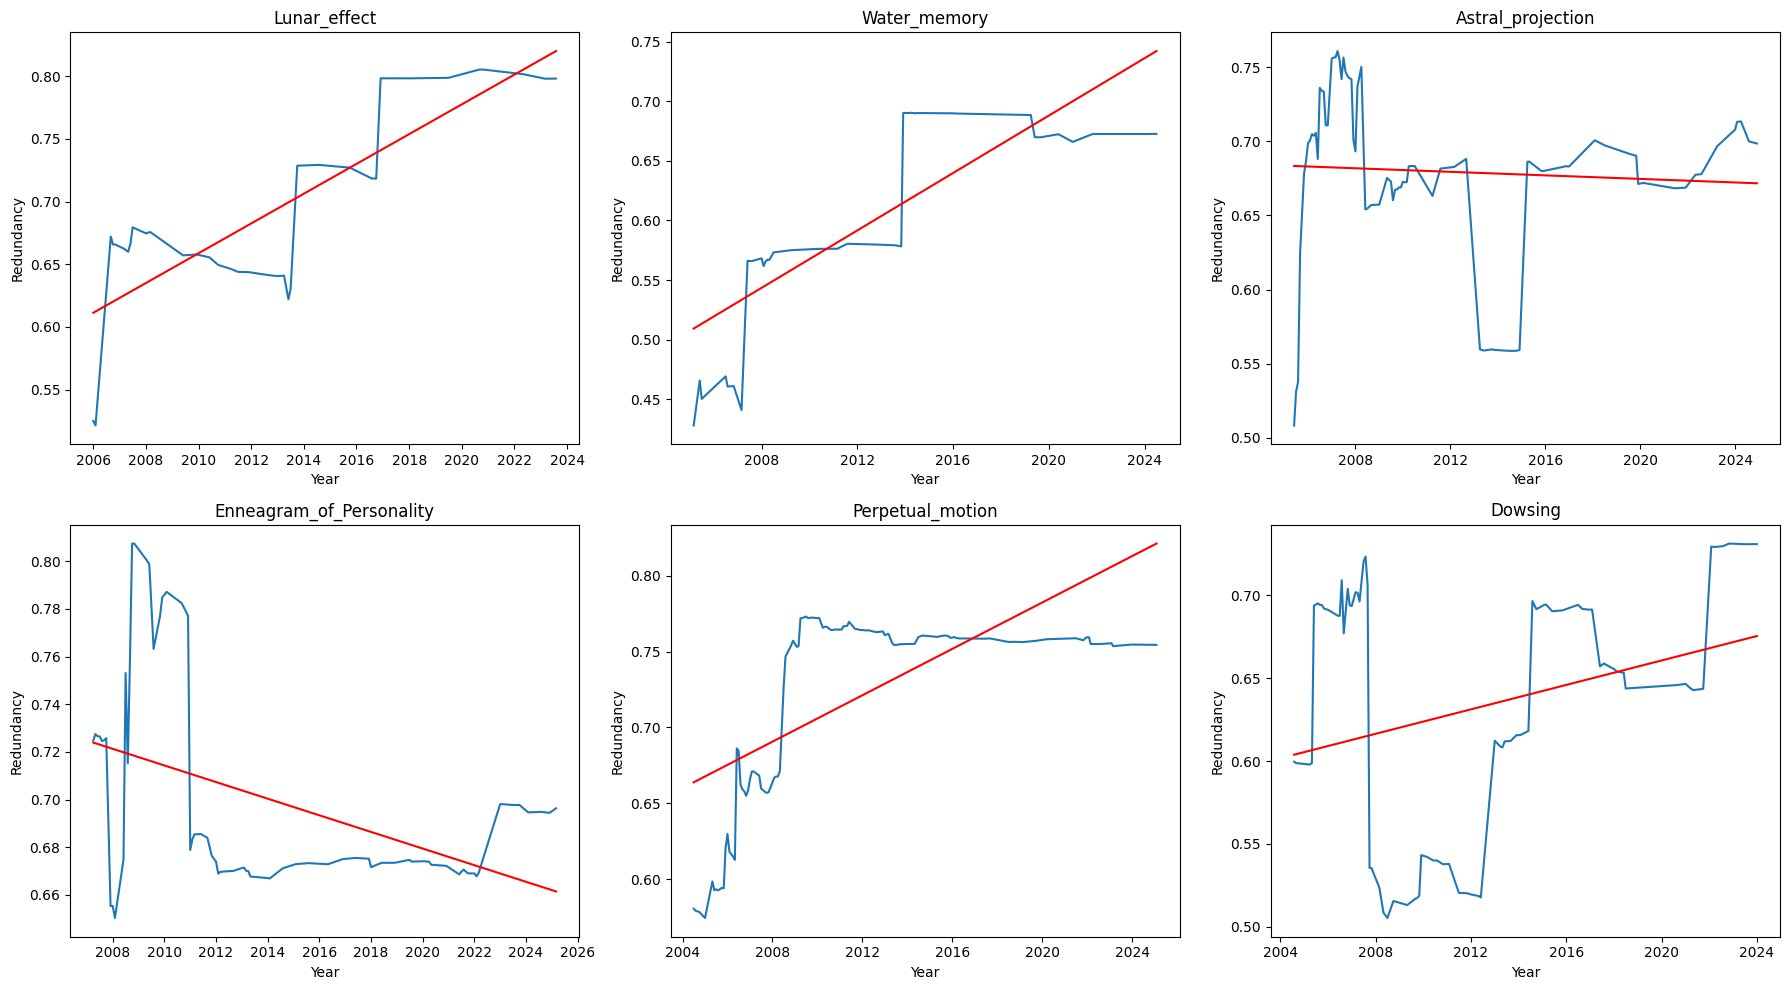
\includegraphics[scale=0.3]{RedundancySixPseudoscientific}
\caption{\label{fig:redundancy_six_pseudoscientific}Evolution of Redundancy in Pseudoscientific Topics}
\end{figure}

Figure \ref{fig:redundancy_six_pseudoscientific} shows the evolution of redundancy for these selected pseudoscientific topics over the past 20 years. As it was the case of scientific topics, redundancy for these topics demonstrates an increasing trend for "Lunar Effect", "Water Memory", "Perpetual Motion", and "Dowsing", and a rather surprising non-increasing trend for "Astral Projection" and "Enneagram of Personality". This decrease in redundancy for the latter two topics may indicate that their Wikipedia articles have undergone substantial editing aimed at streamlining or simplifying the content.

\begin{figure}[H]
\centering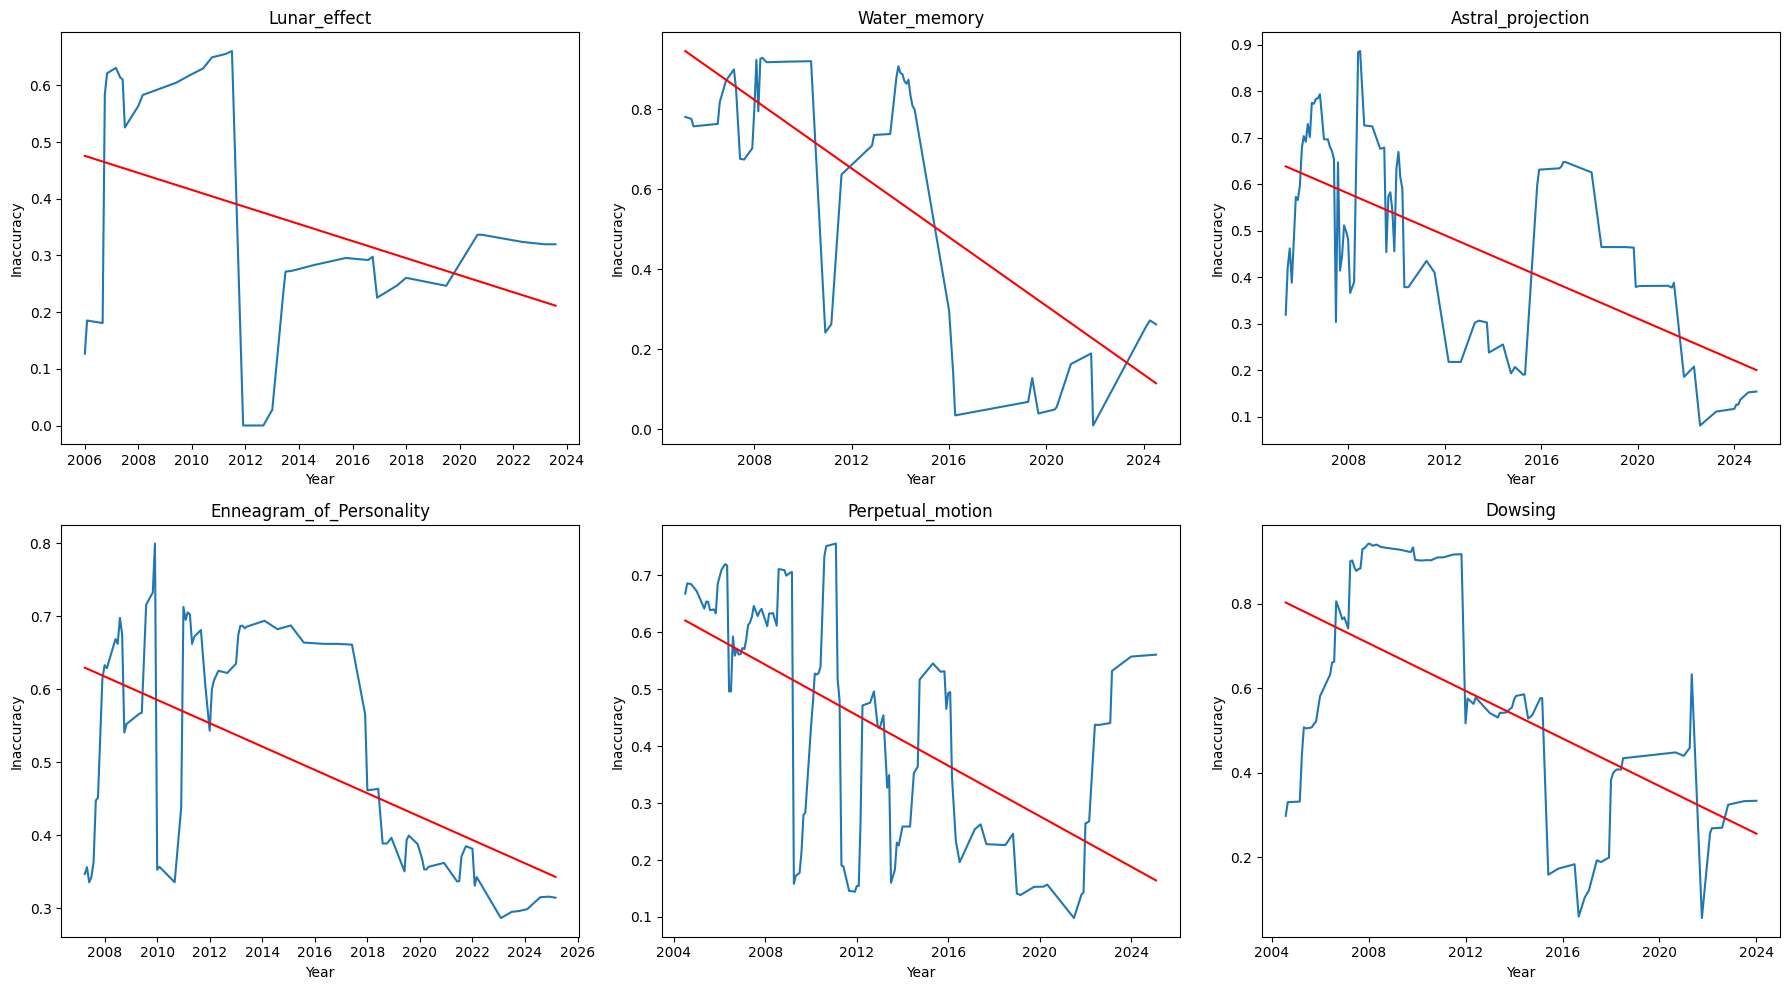
\includegraphics[scale=0.3]{InaccuracySixPseudoscientific}
\caption{\label{fig:inaccuracy_six_pseudoscientific}Evolution of Inaccuracy in Pseudoscientific Topics}
\end{figure}

Figure \ref{fig:inaccuracy_six_pseudoscientific} illustrates the evolution of the estimated inaccuracies for the same pseudoscientific topics. A clear decreasing trend in inaccuracies is observable across most topics, suggesting, somewhat unexpectedly, that controversies regarding these topics have started to settle down. 

\begin{figure}[H]
\centering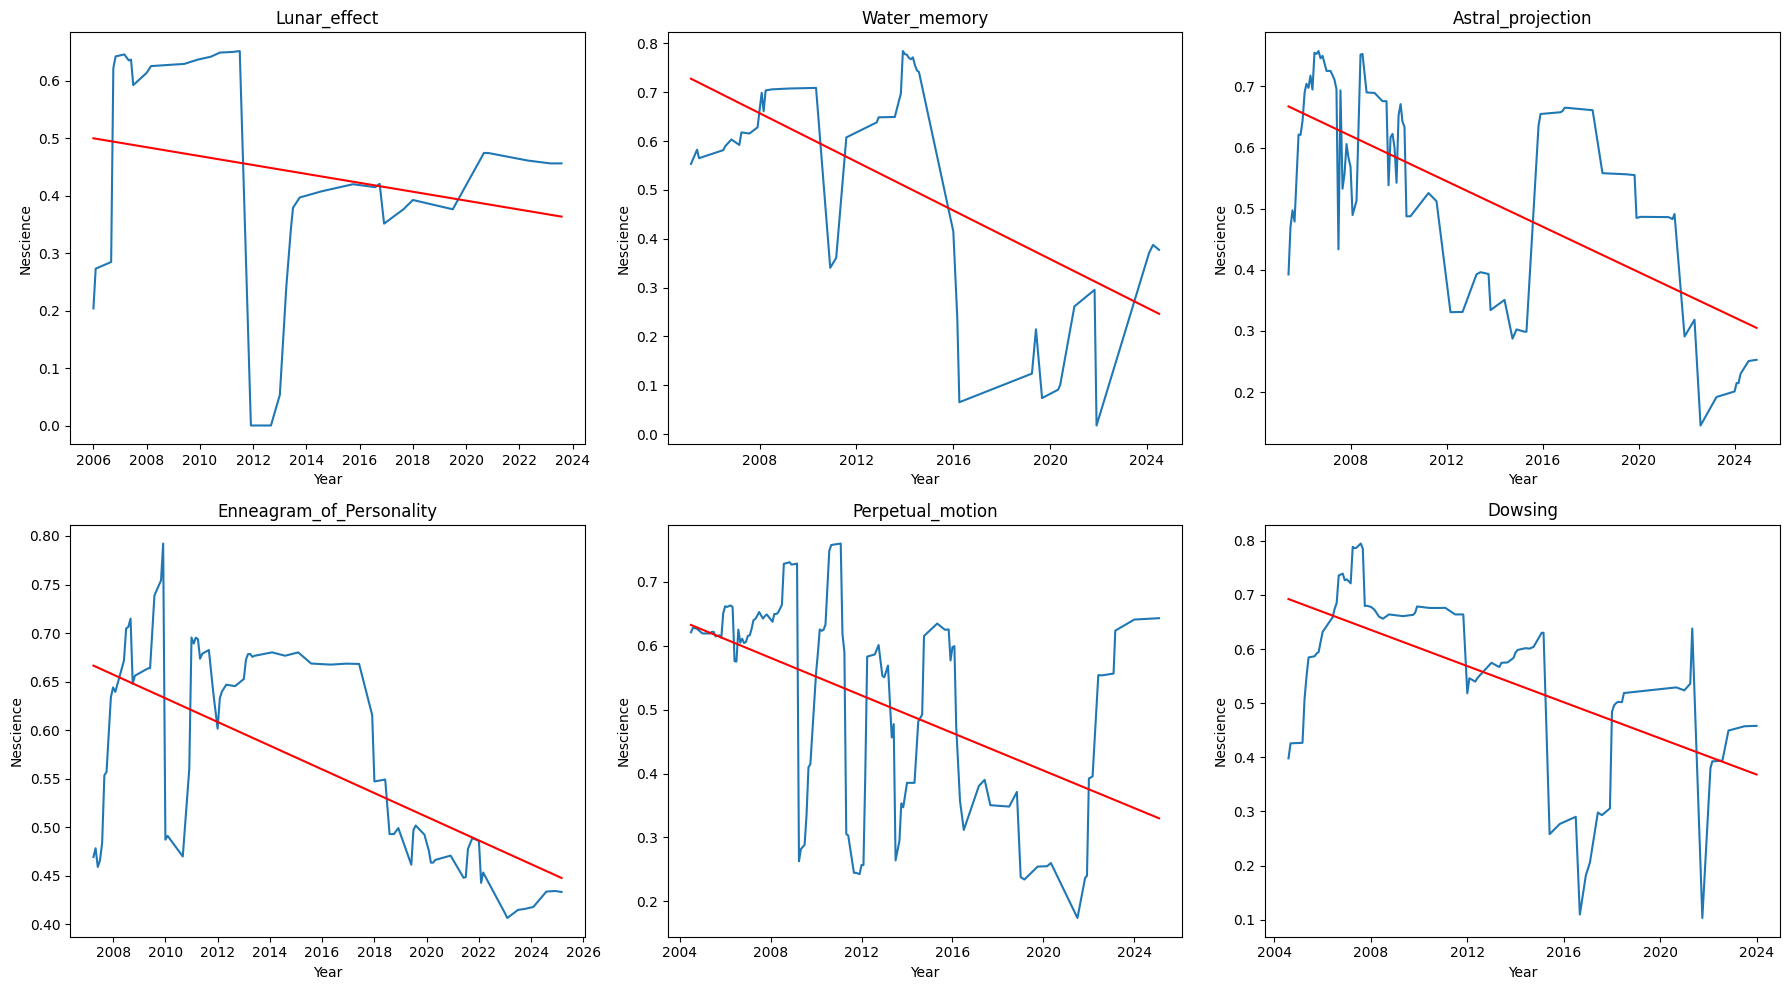
\includegraphics[scale=0.3]{NescienceSixPseudoscientific}
\caption{\label{fig:nescience_six_pseudoscientific}Evolution of Nescience in Pseudoscientific Topics}
\end{figure}

Finally, Figure \ref{fig:nescience_six_pseudoscientific} shows the evolution of the estimated nescience for all selected pseudoscientific topics. As expected, given the previous figures for redundancy and inaccuracy, a decreasing trend is observed for most topics, suggesting that our knowledge about this topics has, in fact, decreased with time.

Our preliminary analysis is too superficial to draw definitive conclusions. A more detailed analysis, employing randomized controlled experiments and rigorous hypothesis testing, needs to be conducted. Additionally, the approximations for redundancy and inaccuracy could be refined further (e.g., citation analysis, scientific community surveys, bibliometric analysis). Based on our initial findings, there appear to be no significant practical differences between science and pseudoscience—both communities seem capable of increasing our knowledge about their respective topics. The essential distinction between science and pseudoscience may lie in the validity and truthfulness of claims, rather than in their methodologies. Alternatively, demarcation could also be based on science's demonstrated capability to transform theoretical results into practical, real-world applications—a capability generally lacking in pseudoscience.

%
% Section: Difficult Research Areas
%
\section{Difficult Research Areas}

In Section {\color{red} ref?} we saw a masure of how difficult is to grasp a research area. In this section we are going to see a measure of how difficult is to grap a individual research topic.

{\color{red} TODO: Study the graspness of a research topic difficult to understand, and the graspness of a easy to understand topic}

%
% Section: Bayesian Approach
%
\section{Bayesian Apprach}

Here I should mention the work of Solomonof with respect to assign a prior probability to theories. I what Solomonof proposed was to use the shortest lenght of programs, what I propose is essentially different, since what I use is lengths of descriptions.


{\color{red} TODO: Study the probability of being true, based on Kolmogorov complexity and unversal probability distributions. Compute the probability of scientific topcis based on the compressed leght of their descriptions.}

{\color{red} TODO: If the acceptability of experimental results is theory-dependent, how can we change the probability of being true of a theory in the presense of new experimental results? There is a high risk of circular argument in the bayesian interpretation of science.}

The Bayesian interpretation of science, based on the Bayes theorem of conditional probabilities, states that the probability that an hypothesis $H$ is true given that an experiment $E$ has been sucessfull, $P(H|E)$, is given by:
\[
P(H|E) = P(H) \frac{ P(E|H) }{ P(E) }
\]
where $P(H)$ is the prior probability of $H$, $P(E|H)$ is the probability of being the experiment sucessfull given that the hypothesis is true, and $P(E)$ is the probability of being true the experiment. In this way, Bayes is a continuous proces in which every sucessfull experiment will increase the probability of $H$ being true, and a failed experiment ({\color{red} How?}) will decrease the probability. The very initian probability $P(H)$, prior to any experiment, is given by the length of its description:
\[
P(H) = r^{l(H)}
\]

\begin{example}
{\color{red} TODO: A real example, with data}
\end{example}

{\color{red} TODO: How my theory of nescience integrates with this?}

{\color{red} TODO: How the base knowledge $a$ affect the probability of the hypothesis $H$?}

{\color{red} TODO: How can we use Bayes and what-if scenaries to improve an hypothesis?}

%
% Section: Inaccuracy-surfeit tradeoff
%
\section{Inaccuracy-sufeit tradeoff}

%
% Section: Effort
%
\section{Effort}

%
% Section: Areas in Decay
%
\section{Areas in Decay}

%
% Section: Perfect Knowledge
%
\section{Perfect knowledge}

Philosophers of science deal with the problem of how knowledge about our world is gathered trough our senses, and if we can trust our perceptions. Also, they address the difficult issue of how knowledge is derived from facts (for example, by means of applying the principle of induction), and if it is sound, from a logic point of view, to make those derivations. Finally, philosophers are interested in how scientific theories are generated based in this knowledge. Any of these problems is covered by the theory of nescience, since we assume that theories (or descriptions in our own terminology) are already known. We do not provide any method to create those theories. What the theory of nescience provides is a set of metrics to quantitatively evaluate, and compare, existing scientific theories. 

It might appear that the descriptions in which the theory of nescience is based are truly objective, in the sense that they must be so clear and well stated that even a computer can reconstruct the original topic given its description. Although this point is true, the problem that prevents the theory to provide an absolute knowledge about our world is the way we choose the entities to study, and how we encode as strings those entities. As we have seen (see Chapter \ref{cha:Topics-and-Descriptions}), the accuracy of our descriptions depend on how good is our encoding of the abstract entities we are studying. Unless the entities are strings themselves, we must assume that our encoding could not be perfect. Moreover, we could be wrong about our assumption that the selected set of entities covers all possible entities of that kind. That is, the set of entities are subject to change as our scientific understanding about them develops. {\color{red} The same might happen in case of encodings.}

Although the theory of nescience does not say anything about how we can reach an absolute knowledge about an entity, it can tell us if we have reached a perfect description (that we make equal to a perfect knowledge). That is, the theory of nescience can answer the question if we have reached a perfect knowledge about a topic, subject that the the entity under study has been properly identified, and the encoding of this entity has no errors.

%
% Section: Unknown Unknown
%
\section{Uknown-unknown}

%
% Section: The Limits of Human Understanding
%
\section{The limits of human understanding}

%
% Section: The Scientific Method
%
\section{The Scientific Method}

The same that we do not try to define what it is a research topic, I do not try to provide an explanation of from where scientific theories come from. According to my interpretation, anything could be a theory, with a initial probability of being true. However, we, as scientists, could clean-up those very unlikely of being true theories.

Although we provide a methodology for the discover of interesting questions, a method to discover what it is hidden in the unknown area, the theory of nescience does not, and does not intend, to be a method (or methodology) for the development of new science. However, in the framework provided by the theory of nescience we could address the problem of which one of the scientific methods proposed so far is more effective to discover new theories. By means of an historical analysis, and by means of analyzing how well the evolution of error and redundancy is covered by the method.

{\color{red} TODO: How non-falsifiable theories are managed by the theory of nescience? What about the desirable property of being as much falsifiable as possible?}

Nescience provides a tool that can be applied to all disciplines. 

Feyerabend aregues that there is no such method, he proposes the principle that "anything goes". anarchistic account of science [...] "increases the freedom of scientists by removing them from methodological constraints"

\emph{Q: How do we evaluate competing scientific theories?}

There exists multiple methods for the comparison of competing scientific theories. Karl Popper's falsificationism is a well known one. According to Popper, scientific theories must be falsifiable, that is, they must be so clearly stated and precise that we can validate them by means of performing an experiment. The more precisely a theory is formulated, and the more accurate its predictions, the better, since that increases the chances of being falsified. As long as the experiments confirm the theory we keep it as valid. However, if a single experiment fails, the theory should be rejected. The main problem of falsificationism is that, in practice, if a experiment fails to confirm a theory, we can not be sure about what went wrong, the experiment or the theory. In the theory of nescience we completely agree with Popper's idea that theories must be clearly stated. In fact, our theories, being Turing machines, are as clearly stated as possible. But, on the contrary of what falsificationism proposes, we do not reject a theory because it has been falsified with an experiment, instead what we propose is to measure the error produced, and take that error into account in our measure of how good is the theory, that is, the nescience of our current best description. Another difference is that, in principle, a theory that makes better prediction is not automatically preferred to another one with less predictability, since we have to take into account not only the error, but also the redundancy of the theory. Unfortunately, in practice, the theory of nescience suffers the same problem than falsificationism, since given that the error of a description must be estimated in practice, usually by means of performing an experiment, we can not be sure if the error is due to the incorrectness of the theory, or due to a wrong designed experiment.

Other alternative interpretations of science, with a stronger orientation towards the theoretical frameworks in which scientific activities take place, like Kuhn's scientific paradigms or Lakatos' research programs, do not have a clear interpretation in the context of the theory of nescience. The same happens when we take into account the social or political aspects of science. Please mind that we are not saying that these possible explanations of science are incorrect. In fact, we have taken seriously the recommendations of Popper, Kuhn, Lakatos and many other philosophers of science during the development of our own theory of nescience.


%
% Section: References
%
\section*{References}

{\color{red} Provide a reference to Wikpedia}

The behavior of compressors depending of the size of objects and window (buffer) size is studied in detail in \cite{cebrian2005common} with applications to the normalized compression distance (a measure of similarity between objects proposed in \cite{li2004similarity}).


